\documentclass[10pt,aspectratio=169]{beamer}

% !TEX TS-program = pdflatex

% -------------------------------------------------
% Fonts (pdflatex-compatible)
% -------------------------------------------------
\usepackage[T1]{fontenc}
\usepackage[utf8]{inputenc}
\usepackage{lmodern}

% -------------------------------------------------
% Base theme
% -------------------------------------------------
\usetheme{default}
\setbeamertemplate{navigation symbols}{}

% Frametitle: flush-left, larger, with a rule underneath
\setbeamertemplate{frametitle}{%
  \nointerlineskip%
  \begin{beamercolorbox}[wd=\paperwidth,ht=2.6ex,dp=1.0ex,leftskip=0.9em]{frametitle}%
    \usebeamerfont{frametitle}\insertframetitle%
  \end{beamercolorbox}%
  \nointerlineskip%
  \begin{beamercolorbox}[wd=\paperwidth,ht=0.35pt,dp=0pt]{framerule}%
  \end{beamercolorbox}%
}

% Footline: slide fraction, bottom-right
\setbeamertemplate{footline}{%
  \hfill%
  \usebeamerfont{footline}%
  \usebeamercolor[fg]{footline}%
  \insertframenumber\,/\,\inserttotalframenumber%
  \hspace{1em}\vspace{0.5em}%
}

% -------------------------------------------------
% Colors: Solarized Light
% -------------------------------------------------
\usepackage{xcolor}
\definecolor{SolBase3} {HTML}{fdf6e3}
\definecolor{SolBase2} {HTML}{eee8d5}
\definecolor{SolBase1} {HTML}{93a1a1}
\definecolor{SolBase00}{HTML}{657b83}
\definecolor{SolBase01}{HTML}{586e75}
\definecolor{SolBlue}  {HTML}{268bd2}
\definecolor{SolCyan}  {HTML}{2aa198}

\setbeamercolor{background canvas}{bg=SolBase3}
\setbeamercolor{normal text}{fg=SolBase00}
\setbeamercolor{alerted text}{fg=SolBlue}
\setbeamercolor{frametitle}{bg=SolBase3, fg=SolBase01}
\setbeamercolor{framerule}{bg=SolBlue}
\setbeamercolor{title}{fg=SolBase01}
\setbeamercolor{subtitle}{fg=SolBase00}
\setbeamercolor{block title}{fg=SolBase3, bg=SolBase01}
\setbeamercolor{block body}{bg=SolBase2, fg=SolBase00}
\setbeamercolor{footline}{fg=SolBase1}
\setbeamercolor{item}{fg=SolBlue}
\setbeamercolor{subitem}{fg=SolCyan}

% -------------------------------------------------
% Packages
% -------------------------------------------------
\usepackage{graphicx}
\usepackage{booktabs}
\usepackage{amsmath}
\usepackage{hyperref}
\hypersetup{
  colorlinks=true,
  linkcolor=SolBlue,
  urlcolor=SolCyan,
  citecolor=SolBlue
}

% -------------------------------------------------
% Typography
% -------------------------------------------------
\usefonttheme{professionalfonts}
\setbeamerfont{frametitle}{size=\large, series=\bfseries}
\setbeamerfont{title}{size=\Large, series=\bfseries}
\setbeamerfont{subtitle}{size=\normalsize}
\setbeamerfont{footline}{size=\scriptsize}
\setlength{\parskip}{0.4em}
\linespread{1.05}
\renewcommand{\arraystretch}{1.2}
\setbeamerfont{caption}{size=\small}
\setbeamercolor{caption name}{fg=SolBase01}

% -------------------------------------------------
% Macros
% -------------------------------------------------
\newcommand{\highlight}[1]{\textcolor{SolBlue}{\textbf{#1}}}
\newcommand{\source}[1]{\vspace{0.4em}\hfill{\scriptsize\textcolor{SolBase1}{#1}}}
\newcommand{\takeaway}[1]{%
  \vspace{0.6em}
  \begin{block}{Takeaway}#1\end{block}
}

% -------------------------------------------------
% Title
% -------------------------------------------------
\title{Projects, Papers, and Proteins}
\subtitle{Do student iGEM projects predict local academic research in synthetic biology?}
\author{Zakh Roth}
\institute{Complexity Science Hub \\ Technical University of Munich}
\date{June 2026}

\begin{document}

% ============================================================
\begin{frame}
  \titlepage
\end{frame}

% ============================================================

\begin{frame}{iGEM: a global natural experiment in distributed innovation}
\begin{columns}[T]
\begin{column}{0.55\textwidth}
  \begin{itemize}
    \item 100k+ participants; 400+ universities; 50+ countries
    \item Teams design organisms around a local problem
    \item Projects, parts, and wiki pages are publicly archived
    \item Runs annually -- a repeated cross-section from 2009 to 2025
  \end{itemize}
\end{column}
\begin{column}{0.42\textwidth}
  \vspace{0.5em}
  {\small\textcolor{SolBase1}{The iGEM corpus gives us a rare window into how student-level scientific interest maps onto local research infrastructure.}}
\end{column}
\end{columns}
\end{frame}

% ============================================================
\begin{frame}{Case Study: Edinburgh 2013}
\begin{columns}[T]
\begin{column}{0.52\textwidth}
  \textbf{The project: \highlight{WastED}}\\[0.3em]
  Engineering \textit{E.\ coli} to produce bioethanol from industrial waste\\[0.3em]
  Core result: enzyme fusion (Pdc--AdhB) raises ethanol yield $\to$
  published in \emph{ACS Synthetic Biology}, 2014\\[0.6em]
  \textbf{Local infrastructure:}
  \begin{itemize}
    \item Advised by Elfick \& French -- both already professors at Edinburgh
    \item Edinburgh ran iGEM teams continuously 2009--2025
  \end{itemize}
\end{column}
\begin{column}{0.45\textwidth}
  \vspace{0.3em}
  \textbf{12 students; where are they now?}
  \begin{itemize}
    \item \highlight{4 pursued PhDs} (Edinburgh, Cambridge, UCL)
    \item \highlight{1 faculty} (asst.\ professor, plant biotech, Krakow)
    \item \highlight{3 moved into biotech industry} (Novonesis, Abbott, Meridian)
    \item \highlight{1 startup founder} (Biotangents Ltd, diagnostics)
    \item 1 commercialisation director (Stevenage Bioscience Catalyst)
    \item $\sim$3 no public trace
  \end{itemize}
\end{column}
\end{columns}


\end{frame}


\begin{frame}{Are student projects topically embedded in local research?}
\begin{columns}[T]
\begin{column}{0.54\textwidth}
  \textbf{Inspired by:}
  \begin{itemize}
    \item Hidalgo et al. (2007): revealed comparative advantage and product space
    \item Neffke \& Henning (2013): skill-relatedness from labor flows
  \end{itemize}
  \vspace{0.5em}
  \textbf{Applied here to text, not products or occupations.}
  \vspace{0.5em}
  \begin{itemize}
    \item Unit: city
    \item Similarity: cosine distance in embedding space
    \item Question: do student projects and local papers occupy related regions of semantic space?
  \end{itemize}
\end{column}
\begin{column}{0.43\textwidth}
  \vspace{0.3em}
  \begin{block}{Core hypothesis}
    Innovation follows a local path:\\
    student projects $\to$ papers $\to$ patents\\[0.3em]
    If so: project topics should \emph{lead} paper topics in the same city by a few years.
  \end{block}
\end{column}
\end{columns}
\end{frame}

% ============================================================

\begin{frame}{Data}
\centering
\begin{tabular}{lrrrl}
\toprule
Corpus & Docs & Cities & Years & Source \\
\midrule
Synbio papers & 10{,}402 & 1{,}218 & 1964--2026 & OpenAlex \\
iGEM projects & 4{,}614 & 626 & 2009--2025 & iGEM Registry \\
BioBrick parts & 89{,}060 & 472 & 2009--2025 & iGEM Registry \\
\midrule
\textbf{Analysis sample} & -- & \textbf{387} & -- & cities with both \\
\bottomrule
\end{tabular}

\vspace{0.6em}
{\small Carbon-capture tagged: 294 papers (2.8\%) and 141 projects (3.1\%).}
\end{frame}

\begin{frame}{SPECTER2 embeds scientific text into a citation-informed space}
\begin{columns}[T]
\begin{column}{0.54\textwidth}
  \begin{itemize}
    \item 768-dim vectors; contrastive learning on citation pairs
    \item \textbf{Proximity adapter}: fine-tuned for semantic similarity, not classification
    \item Cached for all 15{,}000 documents; fully reproducible
  \end{itemize}
  \vspace{0.5em}
  \textbf{City representation:}
  \[
    \bar{\mathbf{a}}_c = \frac{1}{|P_c|} \sum_{p \in P_c} \mathbf{e}_p
  \]
  Mean embedding over all docs of type $t$ in city $c$.
\end{column}
\begin{column}{0.43\textwidth}
  \vspace{0.3em}
  \begin{block}{Why SPECTER2?}
    Standard sentence transformers are not calibrated for scientific text. SPECTER2 is trained on 146M citation pairs; documents that co-cite tend to be nearby.
  \end{block}
\end{column}
\end{columns}
\end{frame}

% ============================================================
\section{Local Alignment}

\begin{frame}{90\% of projects are semantically closer to their own city's papers}
  \centering
  
\includegraphics[width=0.88\textwidth]{../figures/project_level_alignment.png}

  \source{n = 3{,}620 projects; cities with $\geq$ 3 papers; $\delta$ = own-city cosine $-$ mean over all other cities}
\end{frame}

\begin{frame}{Local Alignment Statistical Tests}
\centering
\begin{tabular}{lcc}
\toprule
 & Statistic & $p$-value \\
\midrule
Mean $\delta$ (own $-$ other) & $+0.0135$ & \\
Fraction with $\delta > 0$ & $90.6\%$ & \\
One-sample $t$-test & $t = 78.02$ & $< 0.001$ \\
Wilcoxon signed-rank & & $< 0.001$ \\
\bottomrule
\end{tabular}

\vspace{0.6em}
\takeaway{Projects are systematically closer to local papers than to papers anywhere else. The effect is small but extremely consistent.}
\end{frame}

\begin{frame}{DiD: separating stable specialisation from temporal alignment}
  \centering
  
\includegraphics[width=0.88\textwidth]{../figures/did_alignment.png}

  \source{Annual city-year centroids ($\geq$ 2 papers); 1{,}841 projects in DiD sample}
\end{frame}

\begin{frame}{The temporal component is real}
\centering
\begin{tabular}{lccc}
\toprule
 & Own city & Other cities & Local advantage \\
\midrule
Own year   & 0.9123 & 0.8989 & $+0.0135$ \\
Other years & 0.9062 & 0.8953 & $+0.0109$ \\
\midrule
$\Delta$ (temporal) & $+0.0062$ & $+0.0036$ & \\
\midrule
\textbf{DiD} & \multicolumn{3}{c}{$\mathbf{+0.0026}$} \\
\bottomrule
\end{tabular}

\vspace{0.5em}
{\small Stable city specialisation accounts for most of the alignment. The DiD component is small but positive.}
\end{frame}

% ============================================================
\section{Lead-Lag Structure}

\begin{frame}{Projects are semantically ahead of local papers by about 3 years}
  \centering
  
\includegraphics[width=0.88\textwidth]{../figures/lead_lag_profile.png}

  \source{Lag $k$: cosine similarity between project centroid in year $t$ and paper centroid in year $t+k$; bootstrapped 95\% CI}
\end{frame}

\begin{frame}{The lead-lag slope is not a temporal sampling artifact}
  \centering
  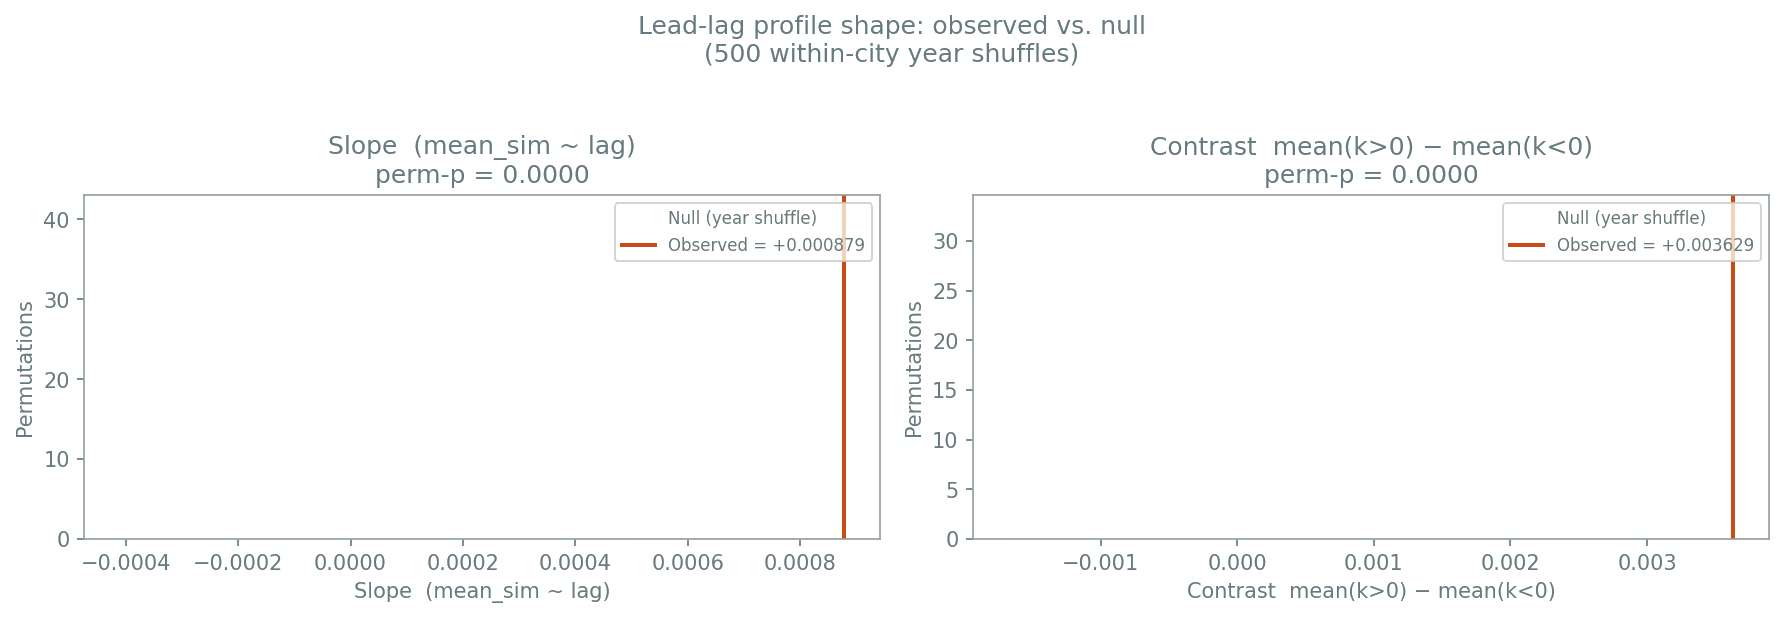
\includegraphics[width=0.88\textwidth]{../figures/lead_lag_permutation.png}

  \source{500 within-city year-shuffles; observed slope = $+0.000879$; null $p_{95}$ = $+0.000246$; perm-$p < 0.05$}
\end{frame}


% ============================================================

% ============================================================
\section{Clusters}

\begin{frame}{UMAP + HDBSCAN finds 83 topic clusters across all 15k documents}
\begin{columns}[T]
\begin{column}{0.52\textwidth}
  \begin{itemize}
    \item UMAP: 60 dimensions, cosine metric
    \item HDBSCAN: 83 clusters, $\sim 20\%$ noise
    \item Cluster overlap = weighted Jaccard on cluster frequency vectors
    \item Sample: 189 cities with $\geq 3$ clustered docs per type
  \end{itemize}
  \vspace{0.5em}
  Mean cluster overlap: $0.081$; median: $0.023$; max: $0.717$
\end{column}
\begin{column}{0.45\textwidth}
  \vspace{0.3em}
  \begin{block}{Why this is better}
    Cluster co-membership is \emph{relative}. It asks: do a city's projects and papers concentrate in the \emph{same topical niches}, not just the same broad field?
  \end{block}
\end{column}
\end{columns}
\end{frame}

\begin{frame}{Cluster co-membership survives the permutation test}
  \centering
  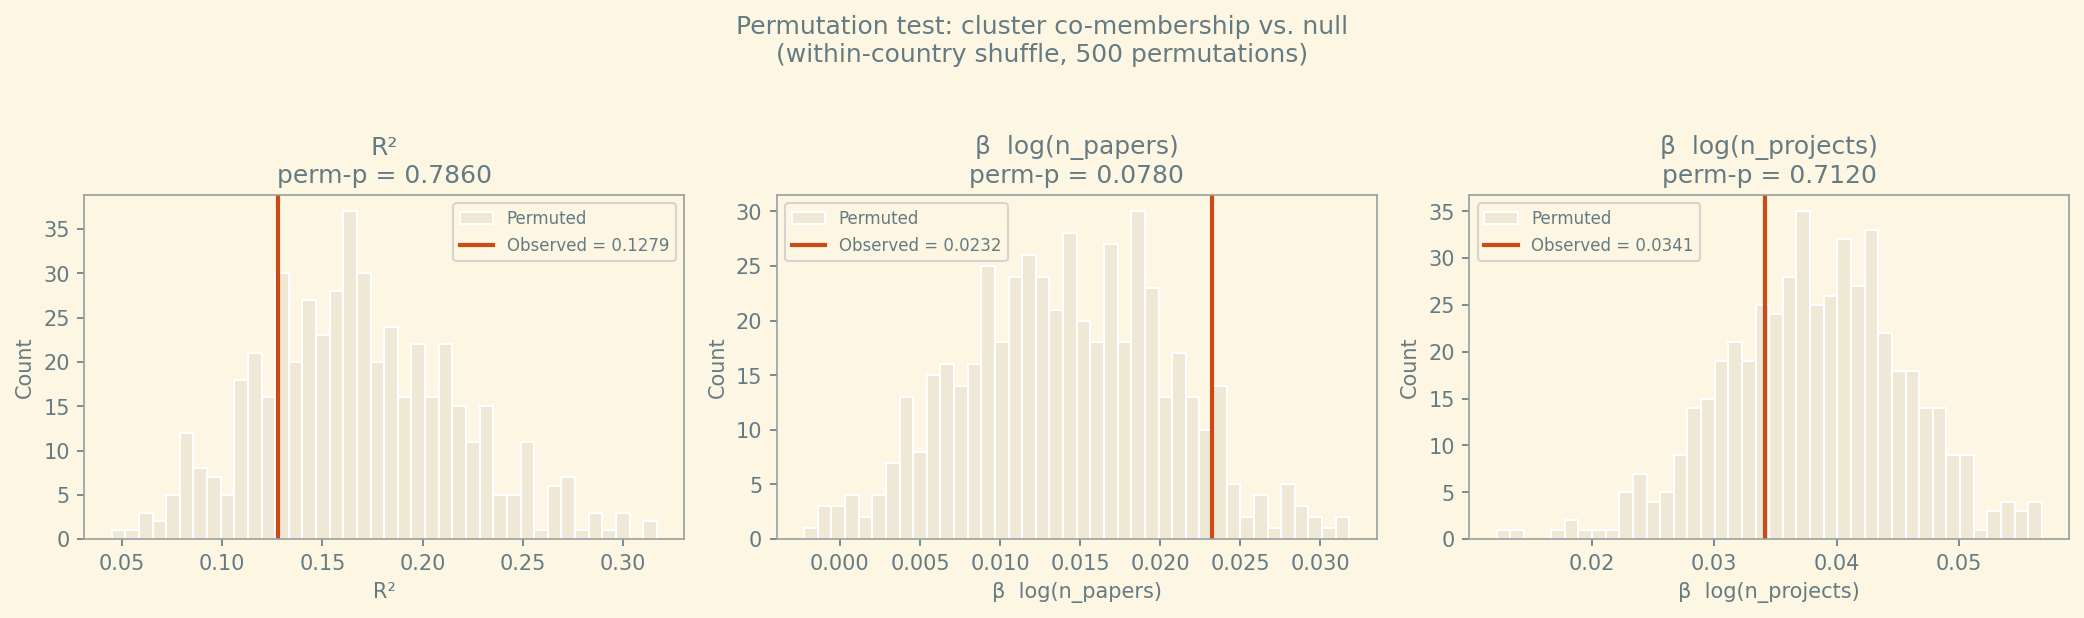
\includegraphics[width=0.88\textwidth]{../figures/permutation_cluster_overlap.png}

  \source{500 within-country shuffles; observed $\beta\ \log n_{\text{projects}} = +0.046^{***}$; perm-$p = 0.03$}
\end{frame}

\begin{frame}{Coefficient plot: cluster co-membership is robust}
  \centering
  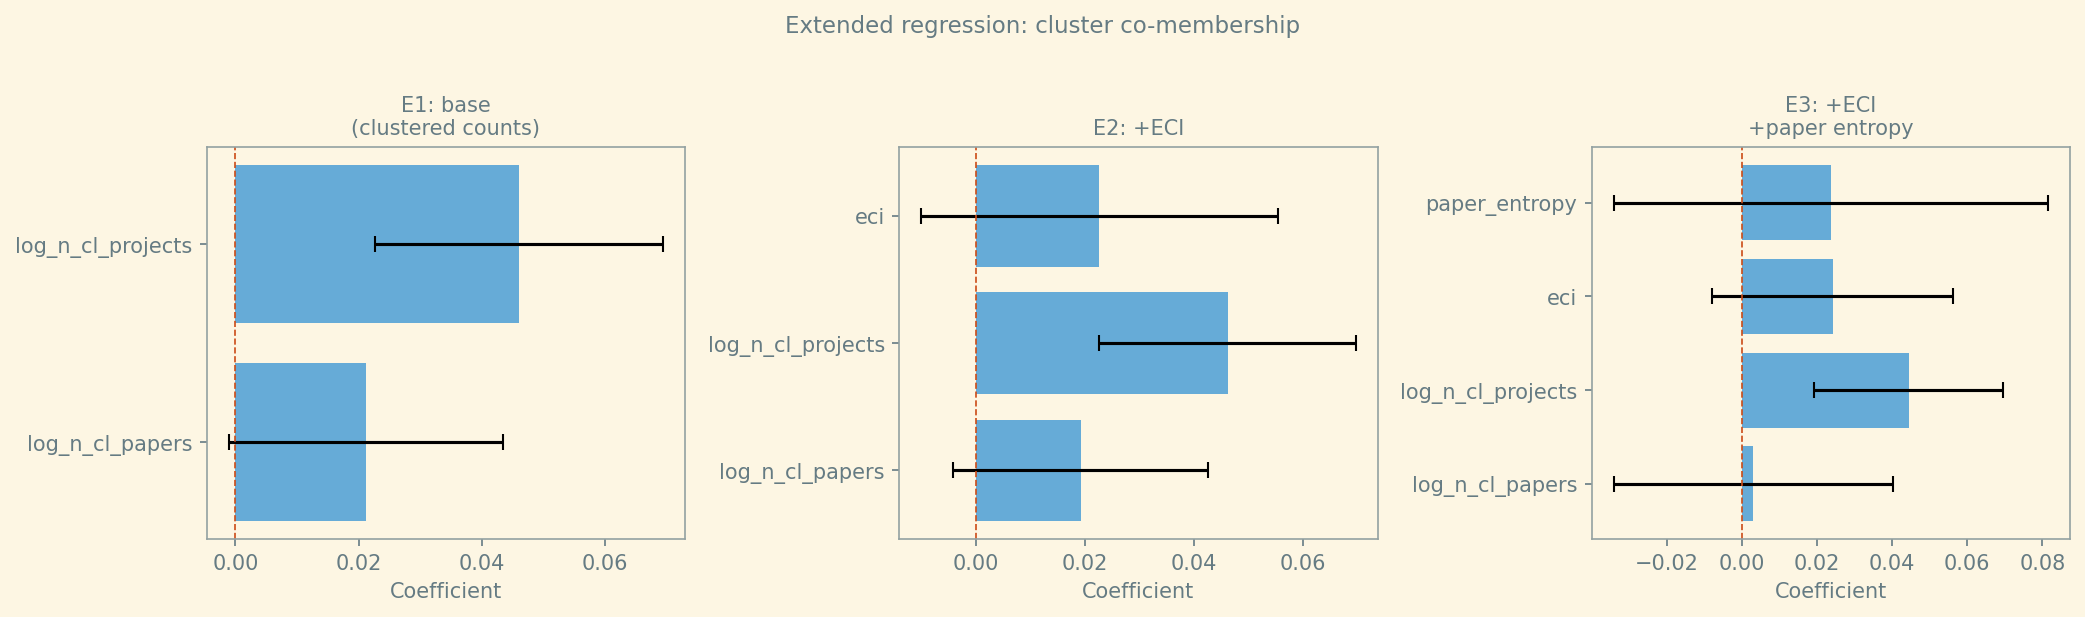
\includegraphics[width=0.88\textwidth]{../figures/coef_plot_extended.png}

  \source{OLS with country FE and robust SE; dependent variable: cluster overlap score}
\end{frame}

% ============================================================
\section{Biobricks: Cross-Modal Validation}

\begin{frame}{Physical part-type composition independently agrees with semantic clusters}
\begin{columns}[T]
\begin{column}{0.52\textwidth}
  BioBrick parts: standardised DNA sequences registered by teams
  \begin{itemize}
    \item Types: promoter, CDS, RBS, terminator, reporter, device, ...
    \item City part-type profile: proportion vector over part types
    \item Shannon entropy measures specialisation
  \end{itemize}
  \vspace{0.5em}
  \textbf{Mantel test:} are part-type distances correlated with cluster-space distances?
\end{column}
\begin{column}{0.45\textwidth}
  \vspace{0.3em}
  \begin{block}{Result (179 cities, 999 permutations)}
    \[r = 0.2207,\quad p < 0.001\]
    Null $p_{95} = 0.073$. Part-type space and semantic cluster space agree.
  \end{block}
\end{column}
\end{columns}
\end{frame}

\begin{frame}{Part-type specialisation varies meaningfully across cities}
  \centering
  
\includegraphics[width=0.88\textwidth]{../figures/part_type_composition.png}

  \source{Top 30 cities by total registered parts; sorted by dominant part type}
\end{frame}

\begin{frame}{Mantel test: part-type and cluster distances are correlated}
  \centering
  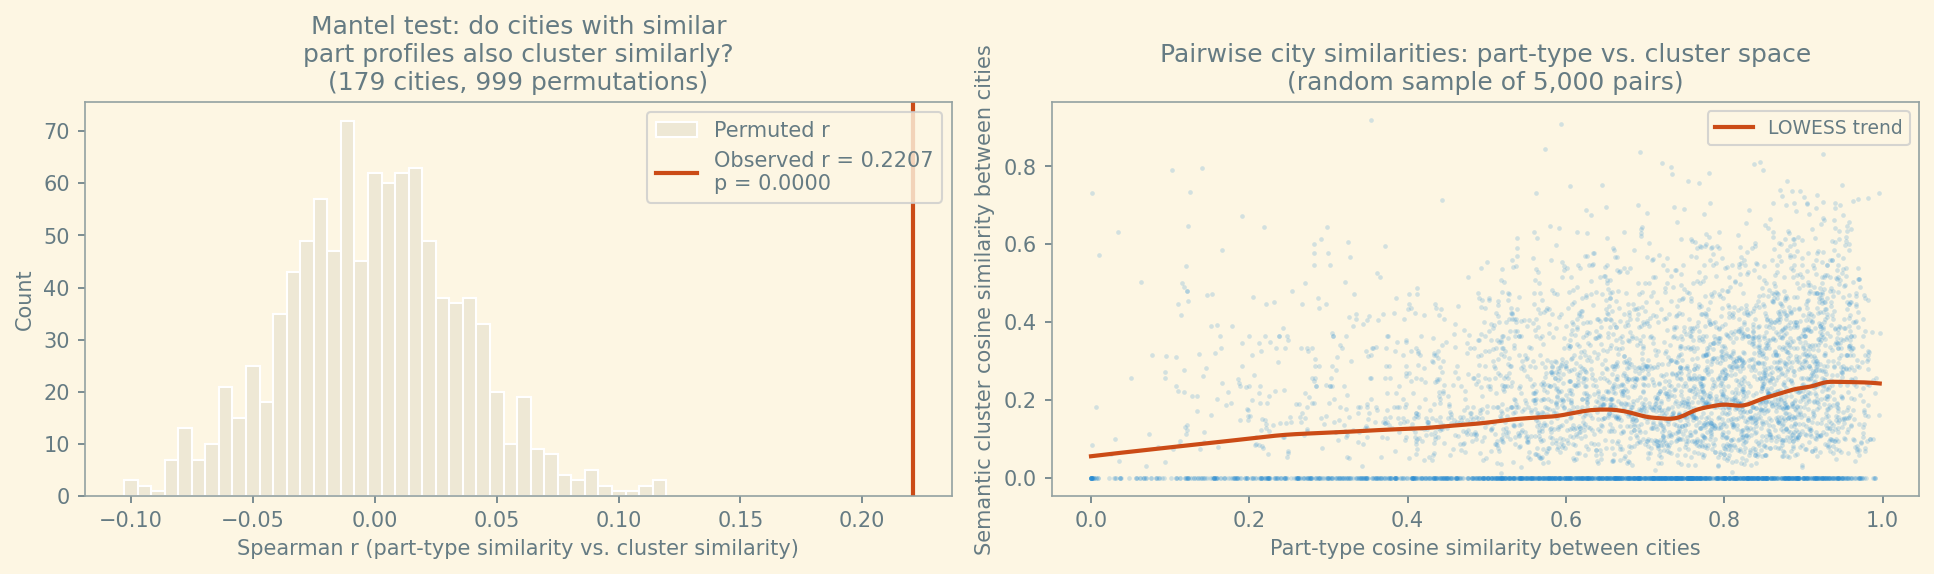
\includegraphics[width=0.88\textwidth]{../figures/mantel_test_parts_vs_cluster.png}

  \source{Spearman Mantel $r = 0.2207$; perm-$p < 0.001$; 179 cities}
\end{frame}

% ============================================================
\section{Summary}

\begin{frame}{Results}
\begin{enumerate}
  \item \textbf{Local alignment is real and consistent} -- 90.6\% of projects are topically closer to their own city's papers ($t = 78$, $p < 0.001$).
  \item \textbf{Projects lead papers by $\approx 3$ years} -- lead-lag peak at $k = +3$; profile shape non-random under permutation.
  \item \textbf{Cluster co-membership is locally specific} -- survives within-country permutation where centroid similarity does not ($p = 0.03$).
  \item \textbf{Part-type space corroborates semantic space} -- Mantel $r = 0.22$, $p < 0.001$; two independent signals agree.
\end{enumerate}
\end{frame}

\begin{frame}{Limitations and what comes next}
\begin{columns}[T]
\begin{column}{0.52\textwidth}
  \textbf{Current limitations:}
  \begin{itemize}
    \item No causal identification -- shared local environment could drive both
    \item Temporal relationships difficult to estimate due to unclear research timelines
    \item iGEM Projects and papers use different language, SPECTER2 not trained on project data
    \item Patents not yet integrated
  \end{itemize}
\end{column}
\begin{column}{0.45\textwidth}
  \textbf{Next steps:}
  \begin{itemize}
    \item Integrate patent corpus
    \item Research success; connect to citation count for papers and awards for projects
    \item Fine-tune model based on links from biobrick registry (paper-part-project)
    \item Improve interactive semantic space explorer + geographic view
  \end{itemize}
\end{column}
\end{columns}
\end{frame}

\begin{frame}{Takeaway}
\begin{block}{}
  In cities with active iGEM participation, the topics that student teams work on are semantically related to the topics that local researchers publish on -- and this co-location in semantic space is not explained by city size alone, holds at the topic-cluster level, and is corroborated by an independent physical signal (BioBrick part-type composition). iGEM projects also tend to share the most similarity with regional research 3 years in the *future*. Causal relationships are not proven; whether this reflects knowledge spillovers, shared local opportunity, or selection of students into research-active cities remains open.
\end{block}
\end{frame}


\end{document}
